\documentclass[11pt]{article}
\usepackage[margin=2.2cm]{geometry}
\usepackage{amsmath}
\usepackage{graphicx}
\usepackage{float}
\usepackage{array}
\usepackage{xcolor}
\usepackage{tabularx}
\usepackage{longtable}
\usepackage[colorlinks=true,linkcolor=blue,urlcolor=blue]{hyperref}
\usepackage{parskip}

\newcommand{\bl}[1]{\textcolor{blue!65!black}{#1}}
\newcommand{\rd}[1]{\textcolor{red!70!black}{#1}}
\newcolumntype{C}{>{\centering\arraybackslash}p{1.45cm}}

\title{\textbf{Weather System Impact --- 8v8 Density Sim}\\[2pt]
\large Tempest Fauna Trail}
\author{Generated by \texttt{tools/simulation/weather\_impact.py}}
\date{2026-06-04}

\begin{document}
\maketitle

\section{Question}

How much do the two weather systems actually swing combat at large team sizes,
as a function of \emph{how many champions are drawn for the live weather affinity}?
The two systems are decoupled in \texttt{src/game/weather\_effects.py}:

\begin{itemize}
  \item \textbf{System A --- Weather Favor} (\texttt{combat\_modifier}): the node
  weather buffs/debuffs each piece by its affinity at combat init. \emph{``Who
  thrives under these conditions?''}
  \item \textbf{System B --- Affinity Clash} (\texttt{damage\_modifier}): a per-hit
  attacker-vs-defender multiplier on the predator/prey ring, weather-independent.
  \emph{``Do I beat this enemy?''}
\end{itemize}

\section{Method}

Teams are size 8. Both sides always draw the \emph{same multiset of tiers}, so the
power budget is equal by construction (power depends only on tier and level); only
the affinity filling each tier-slot varies. \texttt{CLEAR} affinity is inert in
\emph{both} systems (identity Favor, 1.0 Clash), so it is the isolator and filler.

\textbf{Metric.} An 8-piece team spans 8 distinct tiers, so its top piece is
$\sim5\times$ the bottom ($2^{(T-1)/3}$); binary win/loss is then dominated by the
strongest piece's duel and is high variance. The primary read is therefore the
continuous \textbf{HP margin} $m=(\mathrm{hp}_A-\mathrm{hp}_B)/(\mathrm{hp}_A+\mathrm{hp}_B)\in[-1,1]$:
every piece's weather buff feeds it, so the systematic effect surfaces as a
low-variance mean shift. Win\% is reported alongside.

\textbf{Side-bias control.} Each matchup is also played with sides swapped and
folded (margin negated, outcome flipped). This cancels a combat-engine input-order
advantage (Section~\ref{sec:bug}); with it on, identical mirror cells read exactly
$0.000$ margin / $50\%$.

Engine is byte-deterministic; variance comes only from sampling many tier-windows
(seeded). Runs below: System~A/B/AB matrices at 30 samples/cell, density curves at
40 samples/cell, side-swap on.

\section{System A --- Weather Favor vs own-weather density}

Player fields $k$ own-weather (rain) champs $+$ clear fillers against an all-clear
(inert) enemy under rain. The control runs the \emph{same} teams under CLEAR weather
(Favor off); the delta strips champ-design bias, leaving pure Favor.

\begin{center}
\begin{tabular}{r r r r r r r r}
\hline
$k$ & own\% & $m_{\text{favor}}$ & $m_{\text{ctrl}}$ & \textbf{$\Delta m$} & favor\% & ctrl\% & \textbf{$\Delta$win} \\
\hline
0 &   0\% & $+0.000$ & $+0.000$ & $+0.000$ & 50.0 & 50.0 & $+0.0$ \\
1 &  12\% & $+0.183$ & $-0.100$ & $+0.283$ & 60.0 & 45.0 & $+15.0$ \\
2 &  25\% & $+0.300$ & $+0.000$ & $+0.300$ & 65.0 & 50.0 & $+15.0$ \\
3 &  38\% & $+0.267$ & $-0.250$ & $+0.517$ & 63.3 & 36.7 & $+26.7$ \\
4 &  50\% & $+0.133$ & $-0.217$ & $+0.350$ & 56.7 & 40.0 & $+16.7$ \\
5 &  62\% & $+0.583$ & $-0.033$ & $+0.617$ & 78.3 & 48.3 & $+30.0$ \\
6 &  75\% & $+0.350$ & $-0.167$ & $+0.517$ & 68.3 & 43.3 & $+25.0$ \\
7 &  88\% & $+0.567$ & $-0.283$ & $+0.850$ & 80.0 & 36.7 & $+43.3$ \\
8 & 100\% & $+0.383$ & $-0.600$ & \bl{$+0.983$} & 68.3 & 20.0 & \bl{$+48.3$} \\
\hline
\end{tabular}
\end{center}

\textbf{Read.} Full-team Favor swing $\mathbf{+0.98}$ margin / $\mathbf{+48\,pp}$ win
($\pm0.12$ sem). Monotonic in $\Delta m$. Favor is a strong, steadily-accumulating
nudge --- each on-weather piece adds margin.

\section{System B --- Affinity Clash}

CLEAR weather (Favor off); mono-affinity vs mono-affinity. Only the per-hit ring
multiplier differs. Cell $=$ player mean HP margin.

\begin{center}
\begin{tabular}{l|C C C C C}
\textbf{player\,\textbackslash\,enemy} & mist & cloudy & rain & snow & thunder \\
\hline
mist    & $0.000$ & \rd{$-0.967$} & \rd{$-0.967$} & \rd{$-0.083$} & \bl{$+1.000$} \\
cloudy  & \bl{$+1.000$} & $0.000$ & \rd{$-1.000$} & \rd{$-1.000$} & \bl{$+0.867$} \\
rain    & \bl{$+0.967$} & \bl{$+1.000$} & $0.000$ & \rd{$-1.000$} & \rd{$-0.467$} \\
snow    & \rd{$-0.017$} & \bl{$+1.000$} & \bl{$+1.000$} & $0.000$ & \rd{$-0.733$} \\
thunder & \rd{$-1.000$} & \rd{$-0.833$} & \bl{$+0.450$} & \bl{$+0.900$} & $0.000$ \\
\end{tabular}
\end{center}

By ring relation (player vs enemy), aggregated:

\begin{center}
\begin{tabular}{l r r}
\hline
relation & mean margin & win\% \\
\hline
primary\_predator   & \bl{$+0.980$} & \bl{99.0} \\
secondary\_predator & \bl{$+0.640$} & \bl{81.7} \\
secondary\_prey     & \rd{$-0.657$} & \rd{17.3} \\
primary\_prey       & \rd{$-0.940$} & \rd{3.7} \\
\hline
\end{tabular}
\end{center}

\textbf{Read.} At mono-stack saturation, Clash is brutal: a primary-predator team
wins $99\%$, a primary-prey team $4\%$. Antisymmetric ($m(X,Y)\approx-m(Y,X)$),
mirror diagonal exactly 0.

\begin{figure}[H]
\centering
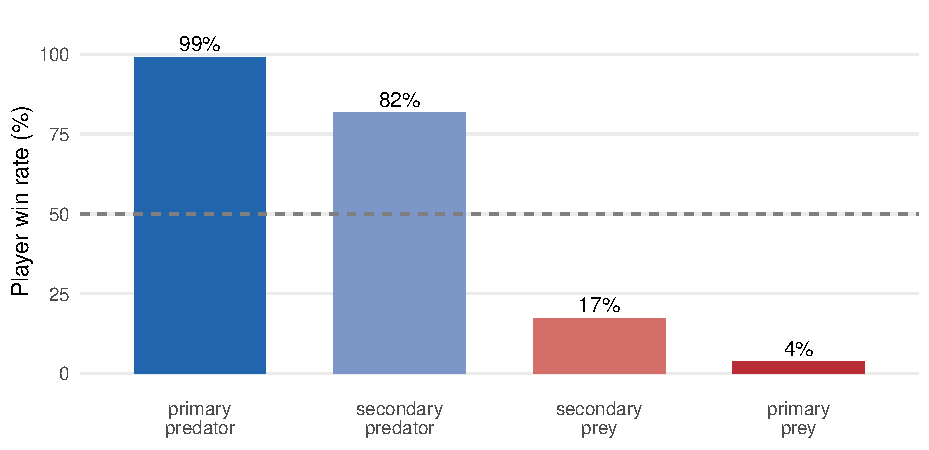
\includegraphics[width=0.82\textwidth]{figs/clash_ring.pdf}
\caption{Affinity Clash at mono-stack saturation: player win rate by ring relation
to the enemy. A wrong-side primary-prey matchup is near-unwinnable irrespective of
weather.}
\end{figure}

\subsection*{Clash intensity vs predator-piece density}

Player ramps $j$ predator pieces $+$ clear filler against a mono-prey enemy, CLEAR
weather, pooled over all 5 ring weathers ($n=400$ at $j{=}8$).

\begin{center}
\begin{tabular}{r r r r r r}
\hline
$j$ & own\% & margin & win\% & $\Delta m$ vs $j{=}0$ & $\Delta$win \\
\hline
0 &   0\% & $+0.482$ & 74.0 & $+0.000$ & $+0.0$ \\
1 &  12\% & $+0.627$ & 81.2 & $+0.145$ & $+7.3$ \\
2 &  25\% & $+0.795$ & 89.8 & $+0.313$ & $+15.7$ \\
3 &  38\% & $+0.795$ & 89.8 & $+0.313$ & $+15.7$ \\
4 &  50\% & $+0.858$ & 92.8 & $+0.375$ & $+18.8$ \\
5 &  62\% & $+0.922$ & 96.0 & $+0.440$ & $+22.0$ \\
6 &  75\% & $+0.950$ & 97.2 & $+0.467$ & $+23.3$ \\
7 &  88\% & $+0.980$ & 99.0 & $+0.497$ & $+25.0$ \\
8 & 100\% & $+0.990$ & 99.5 & \bl{$+0.508$} & \bl{$+25.5$} \\
\hline
\end{tabular}
\end{center}

\textbf{Caveat.} The $j{=}0$ anchor is $74\%$, not $50\%$: at $j{=}0$ this is
clear-roster vs ring-roster (same tiers, different identities) and clear champions
are statlined stronger on average --- a separate roster-balance signal. The
$\Delta m$ column isolates the clash contribution from that bias.

\section{System AB --- both systems live (overlap)}

Node weather $=$ player affinity. Player gets Favor \emph{and} its Clash vs the
enemy. Cell $=$ player mean HP margin.

\begin{center}
\begin{tabular}{l|C C C C C}
\textbf{weather\,\textbackslash\,enemy} & mist & cloudy & rain & snow & thunder \\
\hline
mist    & $0.000$ & \rd{$-1.000$} & \rd{$-0.883$} & \bl{$+0.433$} & \bl{$+1.000$} \\
cloudy  & \bl{$+1.000$} & $0.000$ & \rd{$-1.000$} & \rd{$-0.750$} & \bl{$+1.000$} \\
rain    & \bl{$+1.000$} & \bl{$+1.000$} & $0.000$ & \rd{$-1.000$} & \bl{$+0.100$} \\
snow    & \bl{$+0.467$} & \bl{$+1.000$} & \bl{$+1.000$} & $0.000$ & \rd{$-0.783$} \\
thunder & \rd{$-1.000$} & \rd{$-0.400$} & \bl{$+0.967$} & \bl{$+1.000$} & $0.000$ \\
\end{tabular}
\end{center}

\subsection*{Favor+Clash intensity vs own-affinity density}

Player ramps $j$ own-weather pieces $+$ clear filler vs mono-prey, under weather $X$,
pooled over 5 weathers.

\begin{center}
\begin{tabular}{r r r r r r}
\hline
$j$ & own\% & margin & win\% & $\Delta m$ vs $j{=}0$ & $\Delta$win \\
\hline
0 &   0\% & $+0.667$ & 83.0 & $+0.000$ & $+0.0$ \\
1 &  12\% & $+0.843$ & 92.2 & $+0.175$ & $+9.3$ \\
2 &  25\% & $+0.940$ & 97.0 & $+0.272$ & $+14.0$ \\
3 &  38\% & $+0.968$ & 98.2 & $+0.300$ & $+15.3$ \\
4 &  50\% & $+0.995$ & 99.8 & $+0.328$ & $+16.8$ \\
5 &  62\% & \bl{$+1.000$} & \bl{100.0} & $+0.333$ & $+17.0$ \\
6--8 & $\geq$75\% & $+1.000$ & 100.0 & $+0.333$ & $+17.0$ \\
\hline
\end{tabular}
\end{center}

\textbf{Read.} The systems compound: full mono saturates to $100\%$ win by only
\textbf{$\sim$5/8 on-affinity pieces}. Crucially \textbf{Clash dominates Favor}:
rain under rain still \emph{loses} $0\%$ to snow (snow preys rain) despite the Favor
buff; Favor only fully cancels a \emph{secondary}-prey clash gap (rain vs thunder
$\approx 57\%$).

\section{Cross-system: intensity vs density}

The marginal value of each on-affinity piece, per mechanism. Favor (A) is measured
vs a neutral clear enemy (control-subtracted); Clash (B) and the compound (AB) vs a
mono-prey enemy (vs the $j{=}0$ anchor).

\begin{figure}[H]
\centering
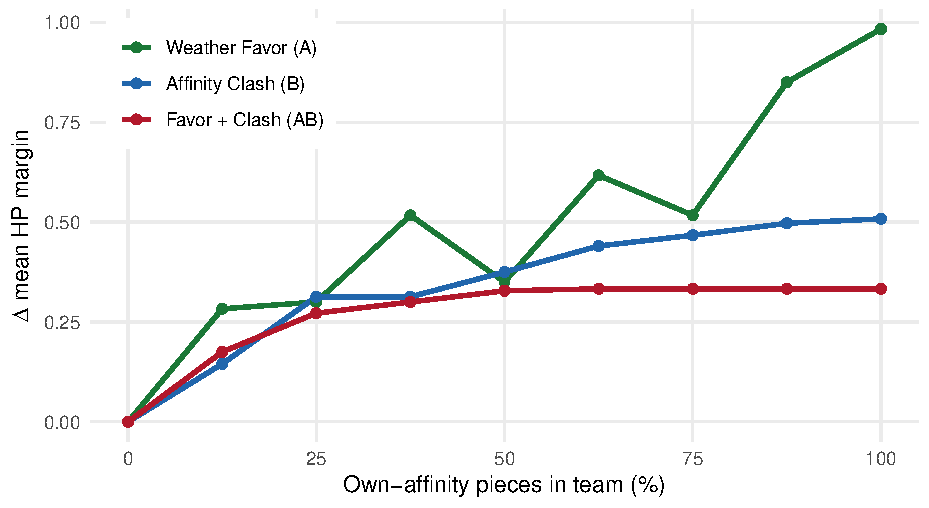
\includegraphics[width=0.92\textwidth]{figs/density_dmargin.pdf}
\caption{$\Delta$ mean HP margin as own-affinity density rises 0--100\%. Read each
curve's \emph{shape}, not cross-curve height: each is measured against a different
baseline (Favor vs a 50\% neutral enemy with full headroom; Clash and compound vs a
high prey-baseline, so they are ceiling-compressed). All grow monotonically; Clash
is the smoothest (low variance), Favor the noisiest (a single dominant top-tier
piece still swings the board, motivating the margin metric).}
\end{figure}

\begin{figure}[H]
\centering
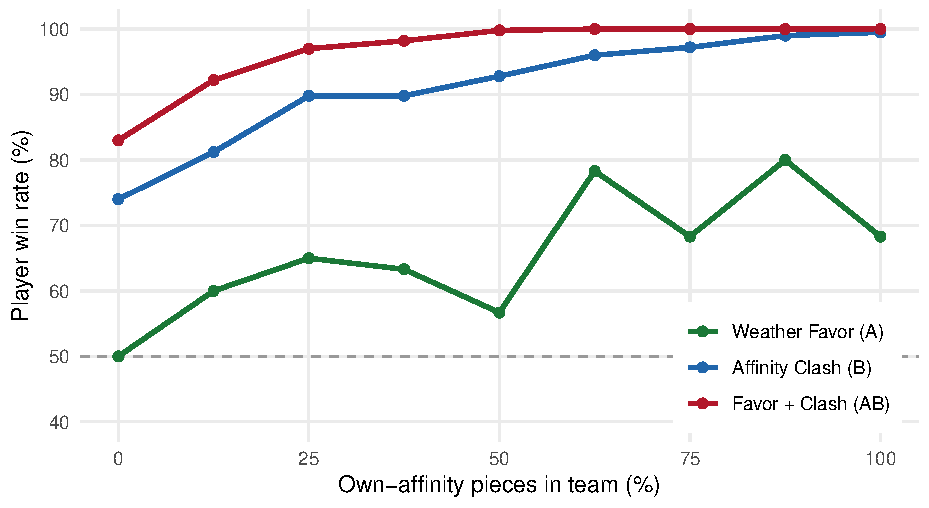
\includegraphics[width=0.92\textwidth]{figs/density_winrate.pdf}
\caption{Absolute player win rate vs density. The compound (AB) reaches 100\% at
$\sim$5/8 pieces. Favor's win\% (A) is noisier and lower-ceilinged than its margin
suggests --- a single dominant top-tier piece can still flip a high-margin board,
which is exactly why margin is the primary metric.}
\end{figure}

\section{Verdict}

\begin{itemize}
  \item Weather matters a lot. Both systems produce large, monotonic swings with
  own-affinity density.
  \item \textbf{Affinity Clash is the harder lever} --- decisive even against an
  opposing Favor buff; a wrong-side primary-prey matchup is near-unwinnable
  ($\sim4\%$) regardless of weather.
  \item \textbf{Weather Favor is a strong but overcomable nudge} ($+48\,pp$ at
  full stack) --- it cancels a secondary clash gap but not a primary one.
  \item Mono-affinity stacking is overwhelming: ceiling at half the team.
\end{itemize}

\section{Side-effect: a combat-engine bug}\label{sec:bug}

The mirror cells reading $\neq 50\%$ before side-swapping exposed a real engine bug.
\texttt{resolve\_combat} (\texttt{combat/legacy.py:469}) sets
\texttt{speed\_tiebreaker = index} over a team-block-then-enemy-block ordering, and
\texttt{\_event\_sort\_key} (\texttt{combat/loop\_new.py:378}) breaks equal
\texttt{attack\_speed} ties by that index. So the entire team out-prioritises the
entire enemy block on any AS tie --- acting, hitting and killing first. An identical
mirror is a \emph{deterministic} side-A win, not a draw. Design intent is
side-independent ordering (first mover by AS and MS only).

This biases every prior combat result and sim report. It is mitigated in this sim
via \texttt{-{}-both-sides} but is \emph{not} fixed in the engine --- a fix changes
the determinism of all existing tests and is a pending decision. Candidate fixes:
interleave tiebreakers (team0, enemy0, team1, \dots) or fold \texttt{move\_speed}
into the tiebreak.

\end{document}
